
\section{App domain}
\label{sec:app-domain}

In order to understand more the domain and study in deep the requirements we tried to use the Domain Driven Development (DDD) technique described by Eric J. Evans \cite{DDD_Eric}. We start with a domain described with Actions that the user could do in the Home screen from the main fab button.
The mains object extends the class Action, they are Chat, ToDoList, Gallery and Geogift. Chat, ToDoList and Gallery have a relation 1 to N with Message, CheckEntry and Photo respectively. The Chat also have a relation 1 to N with ChatDiary that are an entity that group all saved messages from one chat in a precise date, calendar feature use it. 

We use only one type of Message and Photo because this guarantees a more simple interface with Firebase database in the GET and POST operation. Despite of the beneficial use of DDD to understand the requirements and for building a vocabulary of the project domain, the initial model (figure \ref{fig:DDD_model}) doesn't reflect precisely the last implementation of the application and the DDD technique was abandoned due to our lack of discipline.

\begin{figure}[ht]
	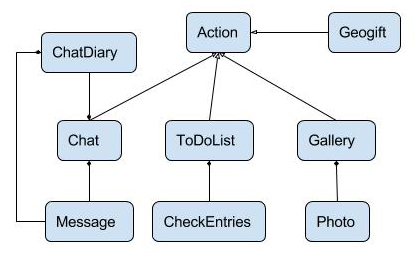
\includegraphics[width=0.50\textwidth]{domain2}
	\caption{Sweetie domain model}
	\label{fig:DDD_model}
\end{figure}